\phantomsection
\subsection{(10\%) Tạo các nhóm người dùng và người dùng}

Để quản lý các bộ phận và người dùng trong công ty, hãy tạo các nhóm
người dùng (group) và người dùng (user) trên server như sau.
Cấp quyền sudo cho người dùng Gia Cát Lượng.

\begin{minipage}{.93\linewidth}
  \centering
  \captionsetup{type=table}
  \caption{\bfseries Danh sách người dùng và nhóm người dùng}
  {\small
    \begin{tabular}{| c | c | c | c | c | c |}
      \hline
      \textbf{STT} & \textbf{Họ tên} & \textbf{Nhóm} & \textbf{Username} & \textbf{Password} & \textbf{Mô tả} \\\hline
      1            & Lưu Bị          & bangiamdoc    & bi.luu            & luubi             & Giám đốc       \\\hline
      2            & Gia Cát Lượng   & bangiamdoc    & luong.giacat      & giacatluong       & Phó giám đốc   \\\hline
      3            & Quan Vũ         & hanhchanh     & vu.quan           & quanvu            & Trưởng phòng   \\\hline
      4            & Trương Phi      & hanhchanh     & phi.truong        & truongphi         & Nhân viên      \\\hline
      5            & Triệu Vân       & banhang       & van.trieu         & trieuvan          & Trưởng phòng   \\\hline
      6            & Mã Siêu         & banhang       & sieu.ma           & masieu            & Nhân viên      \\\hline
      7            & Hoàng Trung     & banhang       & trung.hoang       & hoangtrung        & Nhân viên      \\\hline
    \end{tabular}
  }
\end{minipage}

\phantomsection
\subsubsection{Tạo người dùng}

Trong \texttt{CentOS} để tạo người dùng ta có thể sử dụng lệnh
\texttt{useradd <username>} và dùng lệnh \texttt{passwd <username>}
để đặt mật khẩu cho người dùng. Dưới đây là ví dụ về việc tạo tài khoản
và đặt mật khẩu cho tài khoản Lưu Bị \textit{(\myref{fig:useradd-luubi})}.

\begin{minipage}{.93\linewidth}
  \captionsetup{type=figure, skip=-15pt}
  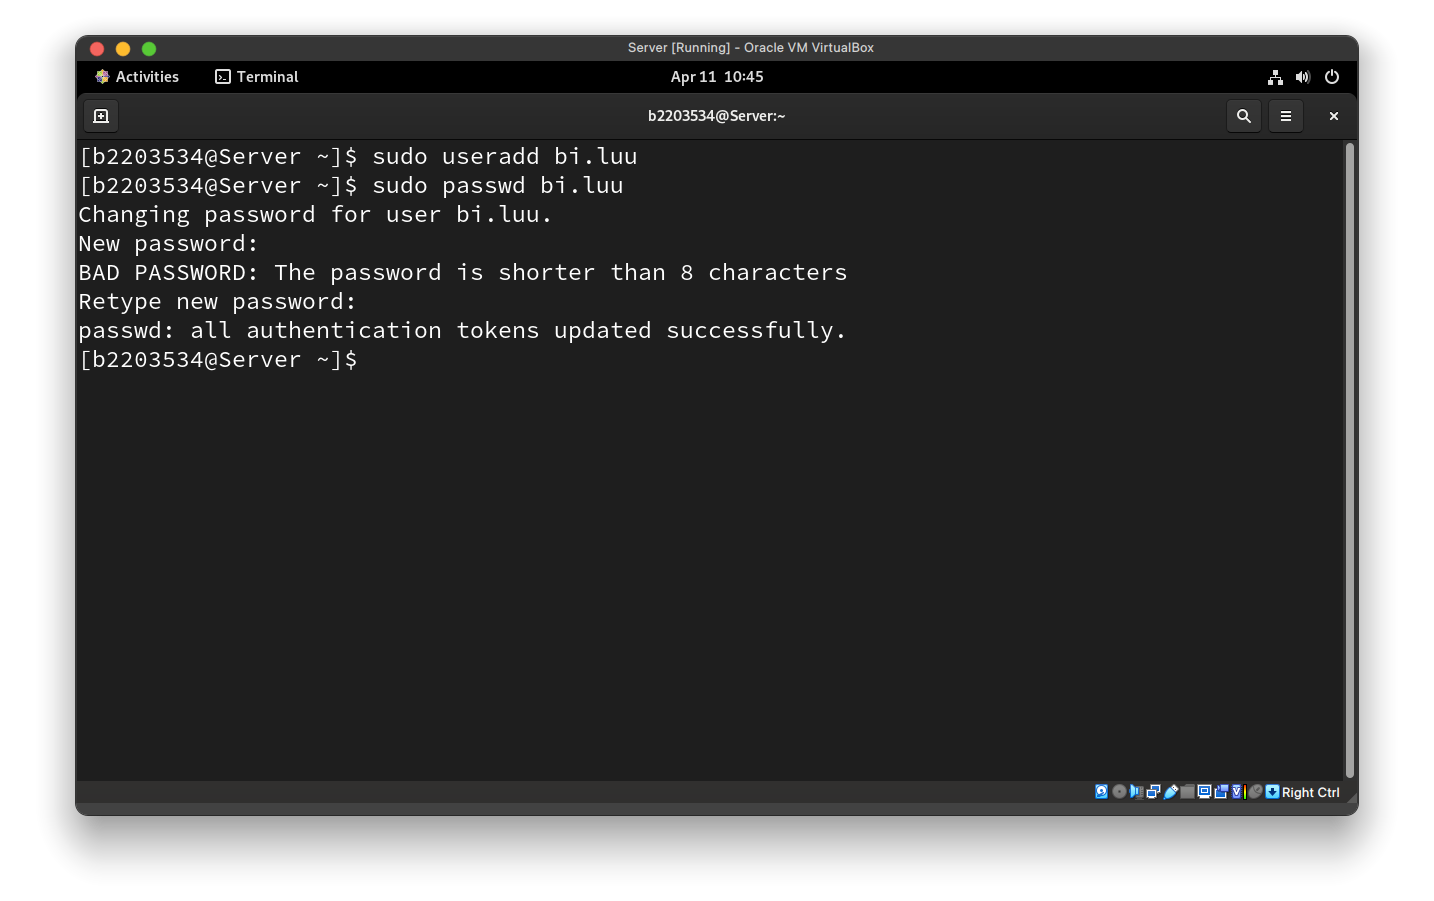
\includegraphics[width=\linewidth]{./imgs/Hinh-12.png}
  \caption{\bfseries Tạo và đặt mật khẩu cho tài khoản Lưu Bị}
  \label{fig:useradd-luubi}
\end{minipage}

\vspace{0.5cm}
\begin{bashlisting}{Tạo và đặt mật khẩu cho tài khoản Lưu Bị}
  sudo useradd bi.luu
  sudo passwd bi.luu
\end{bashlisting}

Các tài khoản còn lại thực hiện tương tự \textit{(\myref{fig:useradd-other})}.

\begin{minipage}{.93\linewidth}
  \captionsetup{type=figure, skip=-15pt}
  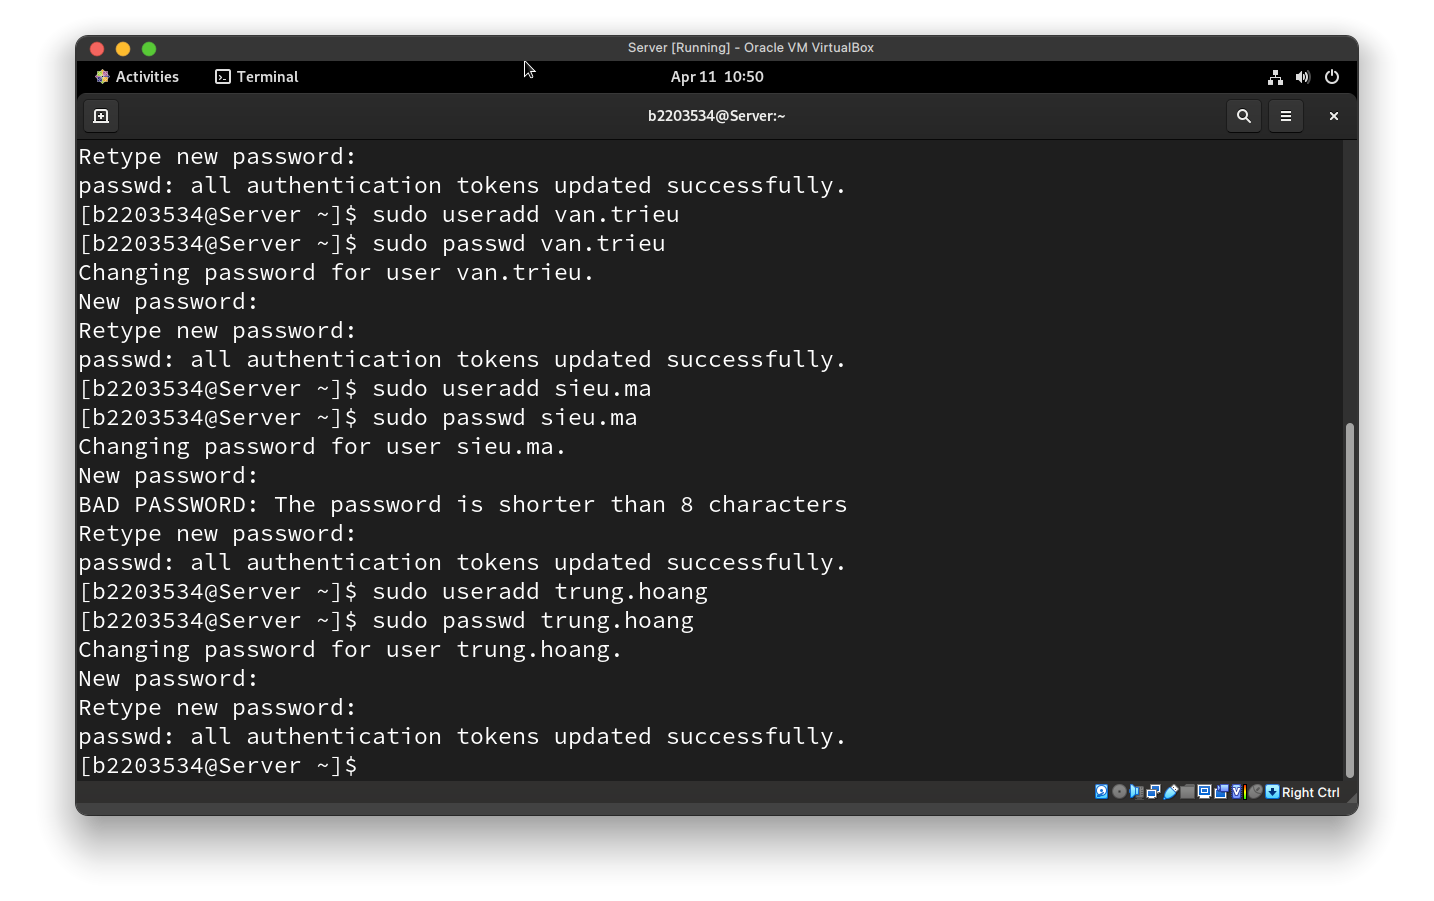
\includegraphics[width=\linewidth]{./imgs/Hinh-13.png}
  \caption{\bfseries Tạo và đặt mật khẩu cho các tài khoản còn lại}
  \label{fig:useradd-other}
\end{minipage}

\vspace{0.5cm}
\begin{bashlisting}{Tạo và đặt mật khẩu cho các tài khoản còn lại}
  sudo useradd bi.luu
  sudo passwd bi.luu
  sudo useradd luong.giacat
  sudo passwd luong.giacat
  sudo useradd vu.quan
  sudo passwd vu.quan
  sudo useradd phi.truong
  sudo passwd phi.truong
  sudo useradd van.trieu
  sudo passwd van.trieu
  sudo useradd sieu.ma
  sudo passwd sieu.ma
  sudo useradd trung.hoang
  sudo passwd trung.hoang
\end{bashlisting}

\phantomsection
\subsubsection{Tạo nhóm người dùng và thêm người dùng vào nhóm}

Ta sử dụng lệnh \texttt{groupadd <group-name>} để thêm nhóm người dùng và thêm người dùng
vào nhóm bằng lệnh \texttt{usermod -aG <group-name> <username>}. Dưới đây là ví dụ tạo
nhóm \texttt{bangiamdoc} và thêm \texttt{luu.bi} và \texttt{luong.giacat} vào
nhóm này \textit{(\myref{fig:groupadd-bangiamdoc})}.

\begin{minipage}{.93\linewidth}
  \captionsetup{type=figure, skip=-15pt}
  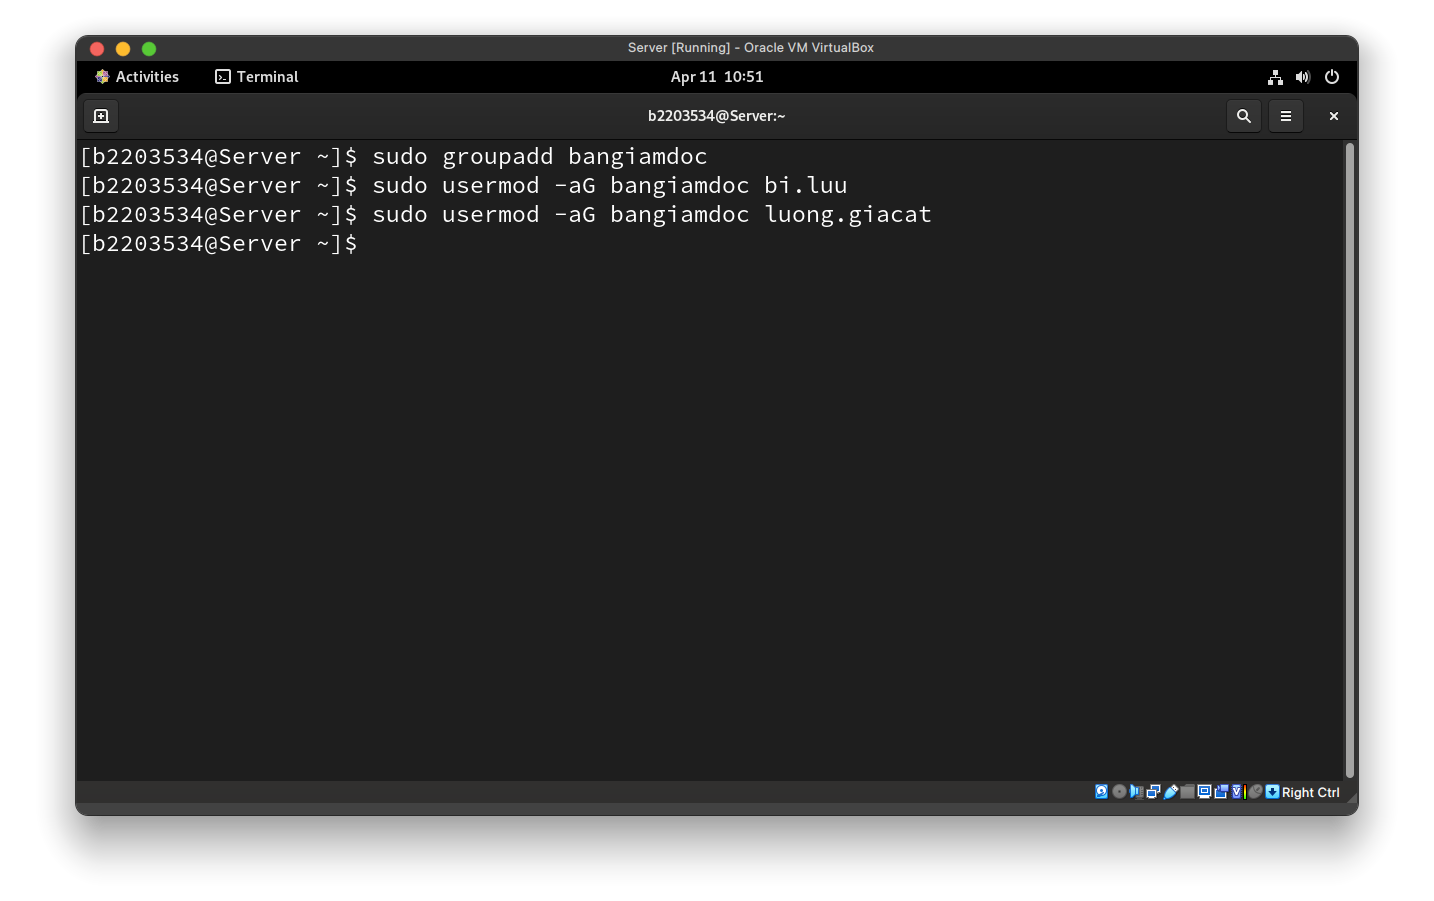
\includegraphics[width=\linewidth]{./imgs/Hinh-14.png}
  \caption{\bfseries Tạo nhóm \texttt{bangiamdoc} và thêm người dùng vào}
  \label{fig:groupadd-bangiamdoc}
\end{minipage}

\vspace{0.5cm}
\begin{bashlisting}{Tạo nhóm \texttt{bangiamdoc} và thêm người dùng vào}
  sudo groupadd bangiamdoc
  sudo usermod -aG bangiamdoc bi.luu
  sudo usermod -aG bangiamdoc luong.giacat
\end{bashlisting}

Các nhóm còn lại thực hiện tương tự \textit{(\myref{fig:groupadd-other})}.

\begin{minipage}{.93\linewidth}
  \captionsetup{type=figure, skip=-15pt}
  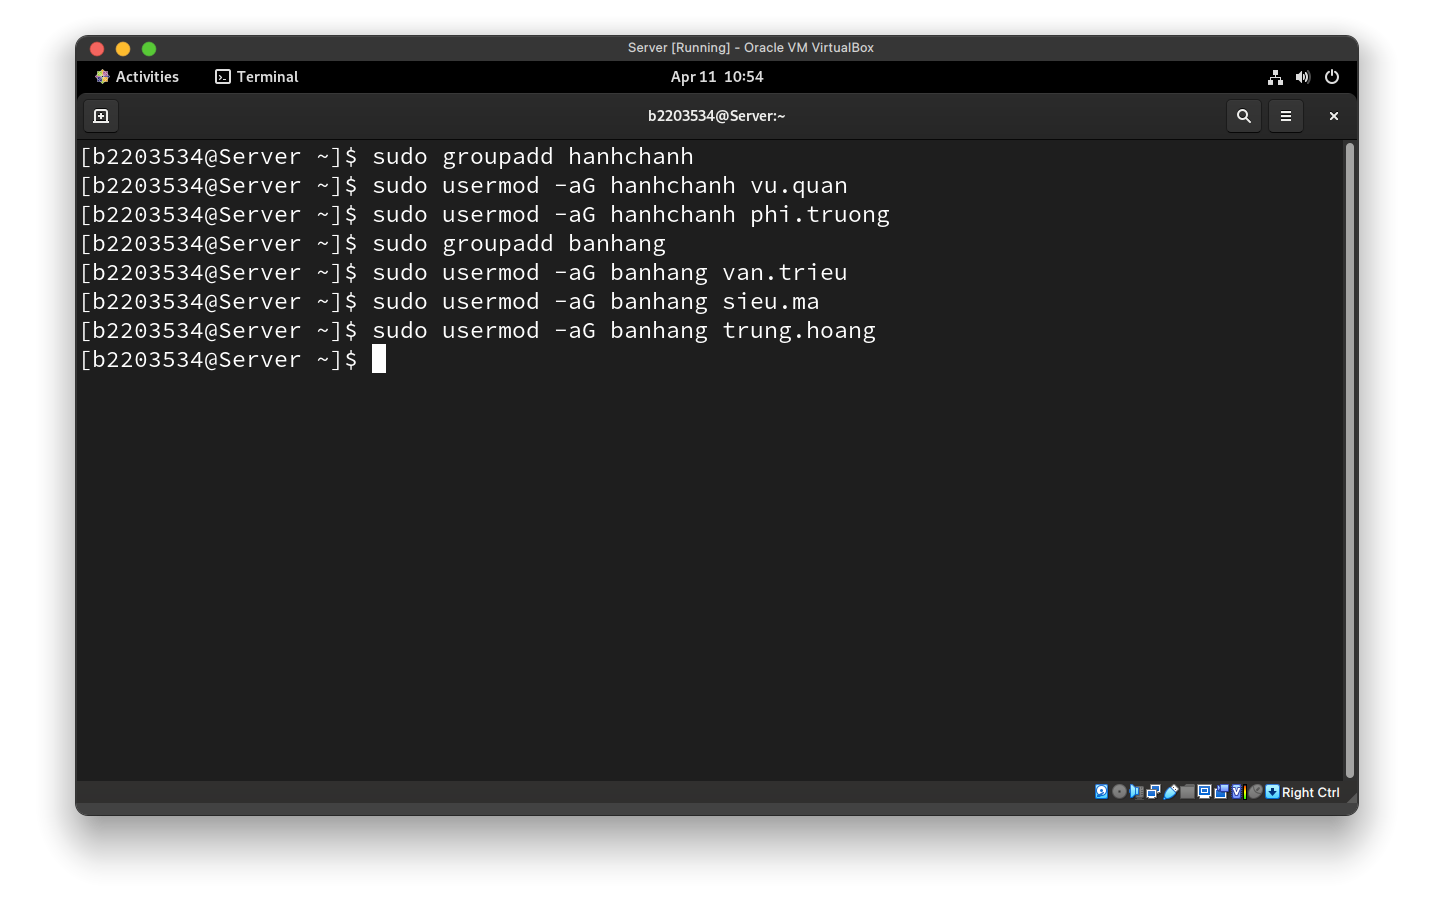
\includegraphics[width=\linewidth]{./imgs/Hinh-15.png}
  \caption{\bfseries Tạo nhóm còn lại và thêm người dùng vào}
  \label{fig:groupadd-other}
\end{minipage}

\vspace{0.5cm}
\begin{bashlisting}{Tạo nhóm còn lại và thêm người dùng vào}
  sudo groupadd hanhchanh
  sudo usermod -aG hanhchanh vu.quan
  sudo usermod -aG hanhchanh phi.truong
  sudo groupadd banhang
  sudo usermod -aG banhang van.trieu
  sudo usermod -aG banhang sieu.ma
  sudo usermod -aG banhang trung.hoang
\end{bashlisting}


\phantomsection
\subsubsection{Cấp quyền sudo cho người dùng Gia Cát Lượng}

Để cấp quyền sudo cho một người dùng, ta thêm người dùng đó nhóm \texttt{sudo} hoặc nhóm
\texttt{wheel}. Bên dưới là minh họa việc thêm người dùng \texttt{luong.giacat} vào nhóm
\texttt{wheel} \textit{(\myref{fig:groupadd-wheel})}.

\begin{minipage}{.93\linewidth}
  \captionsetup{type=figure, skip=-15pt}
  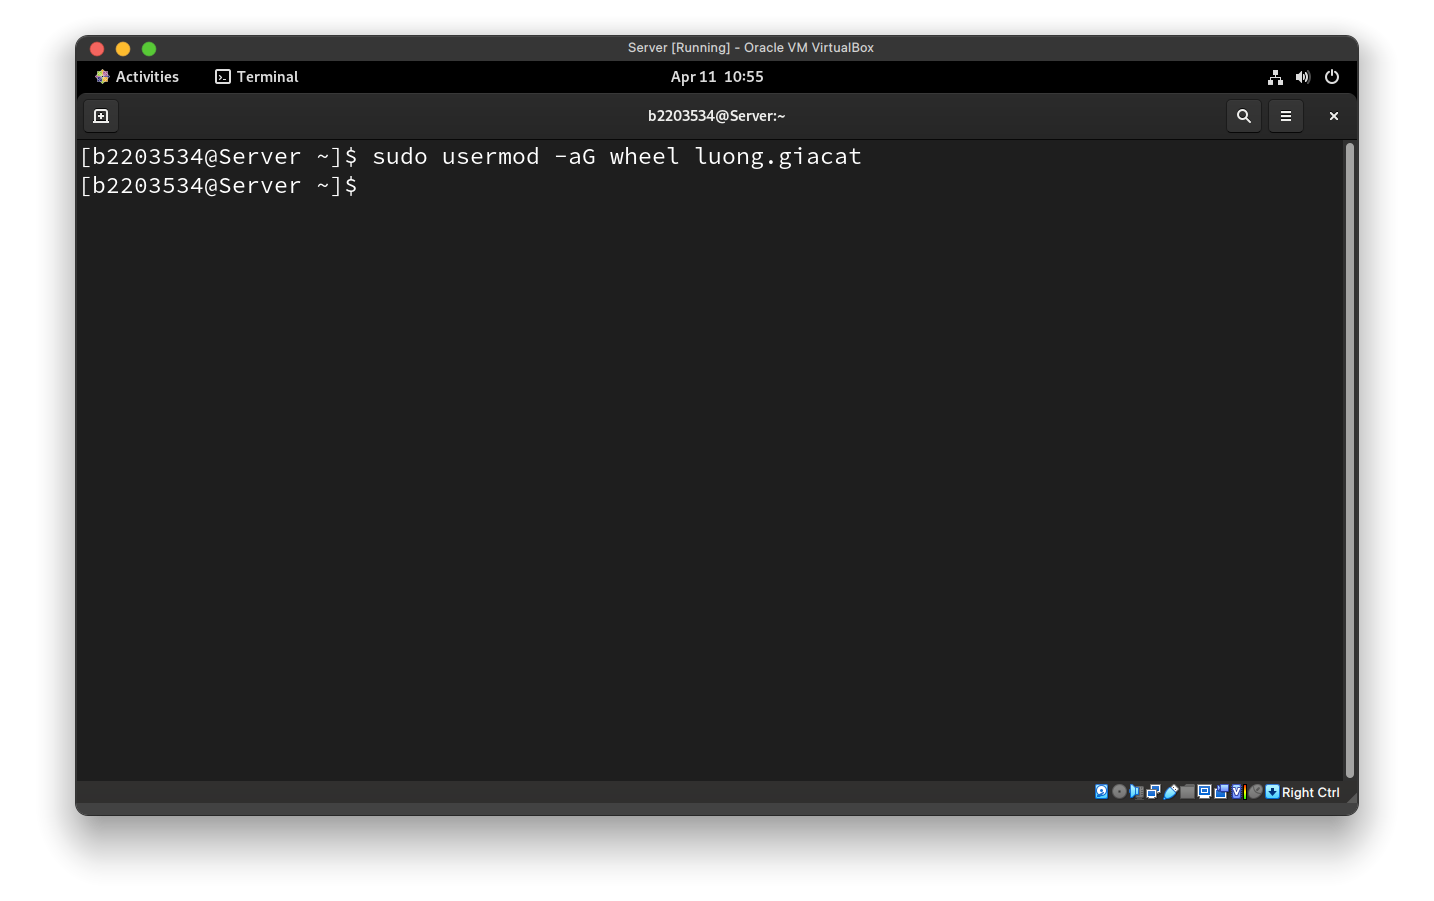
\includegraphics[width=\linewidth]{./imgs/Hinh-16.png}
  \caption{\bfseries Cấp quyền sudo cho người dùng Gia Cát Lượng}
  \label{fig:groupadd-wheel}
\end{minipage}

\vspace{0.5cm}
\begin{bashlisting}{Cấp quyền sudo cho người dùng Gia Cát Lượng}
  sudo usermod -aG wheel luong.giacat
\end{bashlisting}
